%!TEX root = ../thesis.tex
%*******************************************************************************
%****************************** Second Chapter *********************************
%*******************************************************************************

\chapter{Tissue adaptation of T-regulatory cells}

\ifpdf
    \graphicspath{{Chapter2/Figs/Raster/}{Chapter2/Figs/PDF/}{Chapter2/Figs/}}
\else
    \graphicspath{{Chapter2/Figs/Vector/}{Chapter2/Figs/}}
\fi


\section[Introduction]{Introduction}
\label{section2.1}

Regulatory T (Treg) cells, are a specialised CD4+ T cell subset which control immune responses and play a central role in homeostasis (Sakaguchi 2004; Izcue, Coombes, and Powrie 2009). Recent studies have described unique tissue-specific adaptations of non-lymphoid tissue (NLTs) Treg cells distinct from their lymphoid tissue (LT) counterparts. This includes acquisition of an effector phenotype with expression of transcripts encoding effector molecules (Ctla4, Gzmb, Klrg1), chemokines and their receptors (Ccr4), and immunosuppressive cytokines (Il10) (Panduro, Benoist, and Mathis 2016; Bollrath and Powrie 2013), in addition to tissue-specific signature genes associated with their role in each environment (Liston and Gray 2014). Nonetheless, their full transcriptional phenotype and its reflection on NLT population heterogeneity is yet to be uncovered.

Trafficking of T cells to NLTs occurs in steady-state conditions and development (Kimpton et al. 1995; Thome et al. 2015) as well as in response to harmless stimuli at barrier surfaces such as commensal bacteria and dietary antigens (Ivanov et al. 2008). Treg cell migration requires tissue-specific cues involving integrins, chemokine and other G-protein coupled receptors (Cepek et al. 1994; Kim et al. 2013; Chow, Banerjee, and Hickey 2015).

To provide a deeper insight into Treg cell populations in NLTs, we analysed single-cell RNA-seq (scRNA-seq) data of Treg cells from mouse colon and skin, and compared them to LT populations. We identified various transcriptionally distinct clusters of Treg cells in LTs and NLTs, namely a subpopulation in the LTs which showed heavy priming to the NLT environment. Pseudotime ordering of these subpopulations further revealed the transcriptomic adaptations occurring in Treg cells during their transition from the lymph node to barrier tissues. Our results show that these steady-state adaptations share a core signature between bLN-to-skin and mLN-to-colon trajectories, indicative of a general NLT residency programme in barrier tissues. These findings were recapitulated during de novo Treg cell recruitment to melanoma in a murine model system. Lastly, we examined the evolutionarily conservation of NLT Treg cells’ identity between mouse and human.


\section[Results1]{Treg and Tmem cell identity in NLTs is driven by a common expression module}
\label{section2.2}

We performed scRNA-seq on isolated CD4+Foxp3+ (Treg) and CD4+Foxp3-CD44high memory (Tmem) T cells (Figure S1A) from two barrier NLT sites - the colonic lamina propria (hereinafter referred to as colon) and the skin - their lymphoid counterparts in the draining mesenteric and brachial lymph nodes (mLN and bLN), and the spleen from a Foxp3-GFP mouse reporter line (Bettelli et al. 2006) (Figure~\ref{fig:chap2_fig1}A). We will refer to Treg and Tmem cells together as CD4+ T cells. For each sorted population, single-cells were captured using the droplet-based microfluidic system Chromium (10x Genomics), hereinafter referred to as 10x. We obtained 30396 good quality cells (see Methods, Figure S1C, Table S1). Using the same gating strategy, two Smart-seq2 (Picelli et al. 2014) plate-based datasets were produced independently. These confirmed findings drawn from the 10x, and complemented them with higher gene coverage and full T cell receptor (TCR) sequences.

A tSNE projection (Figure~\ref{fig:chap2_fig1}B) after filtering (Figure S1B; Table S2) showed a division between LT and NLT, with cells from LTs divided into two clusters, according to cell-type. NLT cells formed one single skin cluster and two clusters separating Treg and Tmem cells from colon (Figure~\ref{fig:chap2_fig1}B). We defined gene expression signatures for Treg and Tmem cells in peripheral tissues by examining differentially expressed (DE) genes between all NLT and LT cells and, in parallel, between Treg and Tmem cells (Figure~\ref{fig:chap2_fig1}C). NLT T cell populations are characterised by the expression of several elements of the TNFRSF-NF-$\kappa$B pathway, including transducers (\textit{Traf1}, \textit{Traf4}, \textit{Traf2b}), effectors (\textit{Nfkb1}, \textit{Nfkb2}, \textit{Rel}, \textit{Rela}, \textit{Relb}) and inhibitors (\textit{Nfkbib}, \textit{Nfkbid}, \textit{Nfkbie}). In Tmem cells, these were accompanied by cytokines (\textit{Tnfsf8}, \textit{Tnfsf11}) and various pathway inhibitors, such as \textit{Tnfaip8}. In contrast, NLT Treg cells expressed TNF receptors (\textit{Tnfrsf4}, \textit{Tnfrsf9}, \textit{Tnfrsf18}) and transducers (Pim1), underscoring the importance of signalling via the TNFRSF-NF-$\kappa$B axis in controlling Treg cells in the peripheral tissues. Several chemokine receptors appeared DE across tissues and cell types. \textit{Ccr4}, \textit{Ccr8} and \textit{Cxcr4} were upregulated in both colon and skin T cells, while \textit{Ccr1} and \textit{Ccr5} were specific to colon and \textit{Ccr6} to skin. \textit{Cxcr6} was more highly expressed in NLT Tmem cells. We also detected other genes involved in NLT identity (\textit{Crem}, \textit{Rgs2}, \textit{Il1r2}, \textit{Icos}, \textit{Hif1a}, \textit{Kdm6b}, \textit{Gata3}), including some specific to Tmem (\textit{Vps37b}, \textit{Id2}, \textit{Ramp3}, \textit{Tnfsf8}) and Treg cells (\textit{Il10}, \textit{Gzmb}, \textit{Ctla4}, \textit{Cd83}, \textit{Socs2}).

Together, the scRNA-seq datasets collected provide a comprehensive overview of Treg and Tmem cells in multiple lymphoid and non-lymphoid tissues, and identify the TNFRSF-NF-$\kappa$B pathway as key to their barrier tissue identity.

\begin{figure}[htbp!] 
\centering    
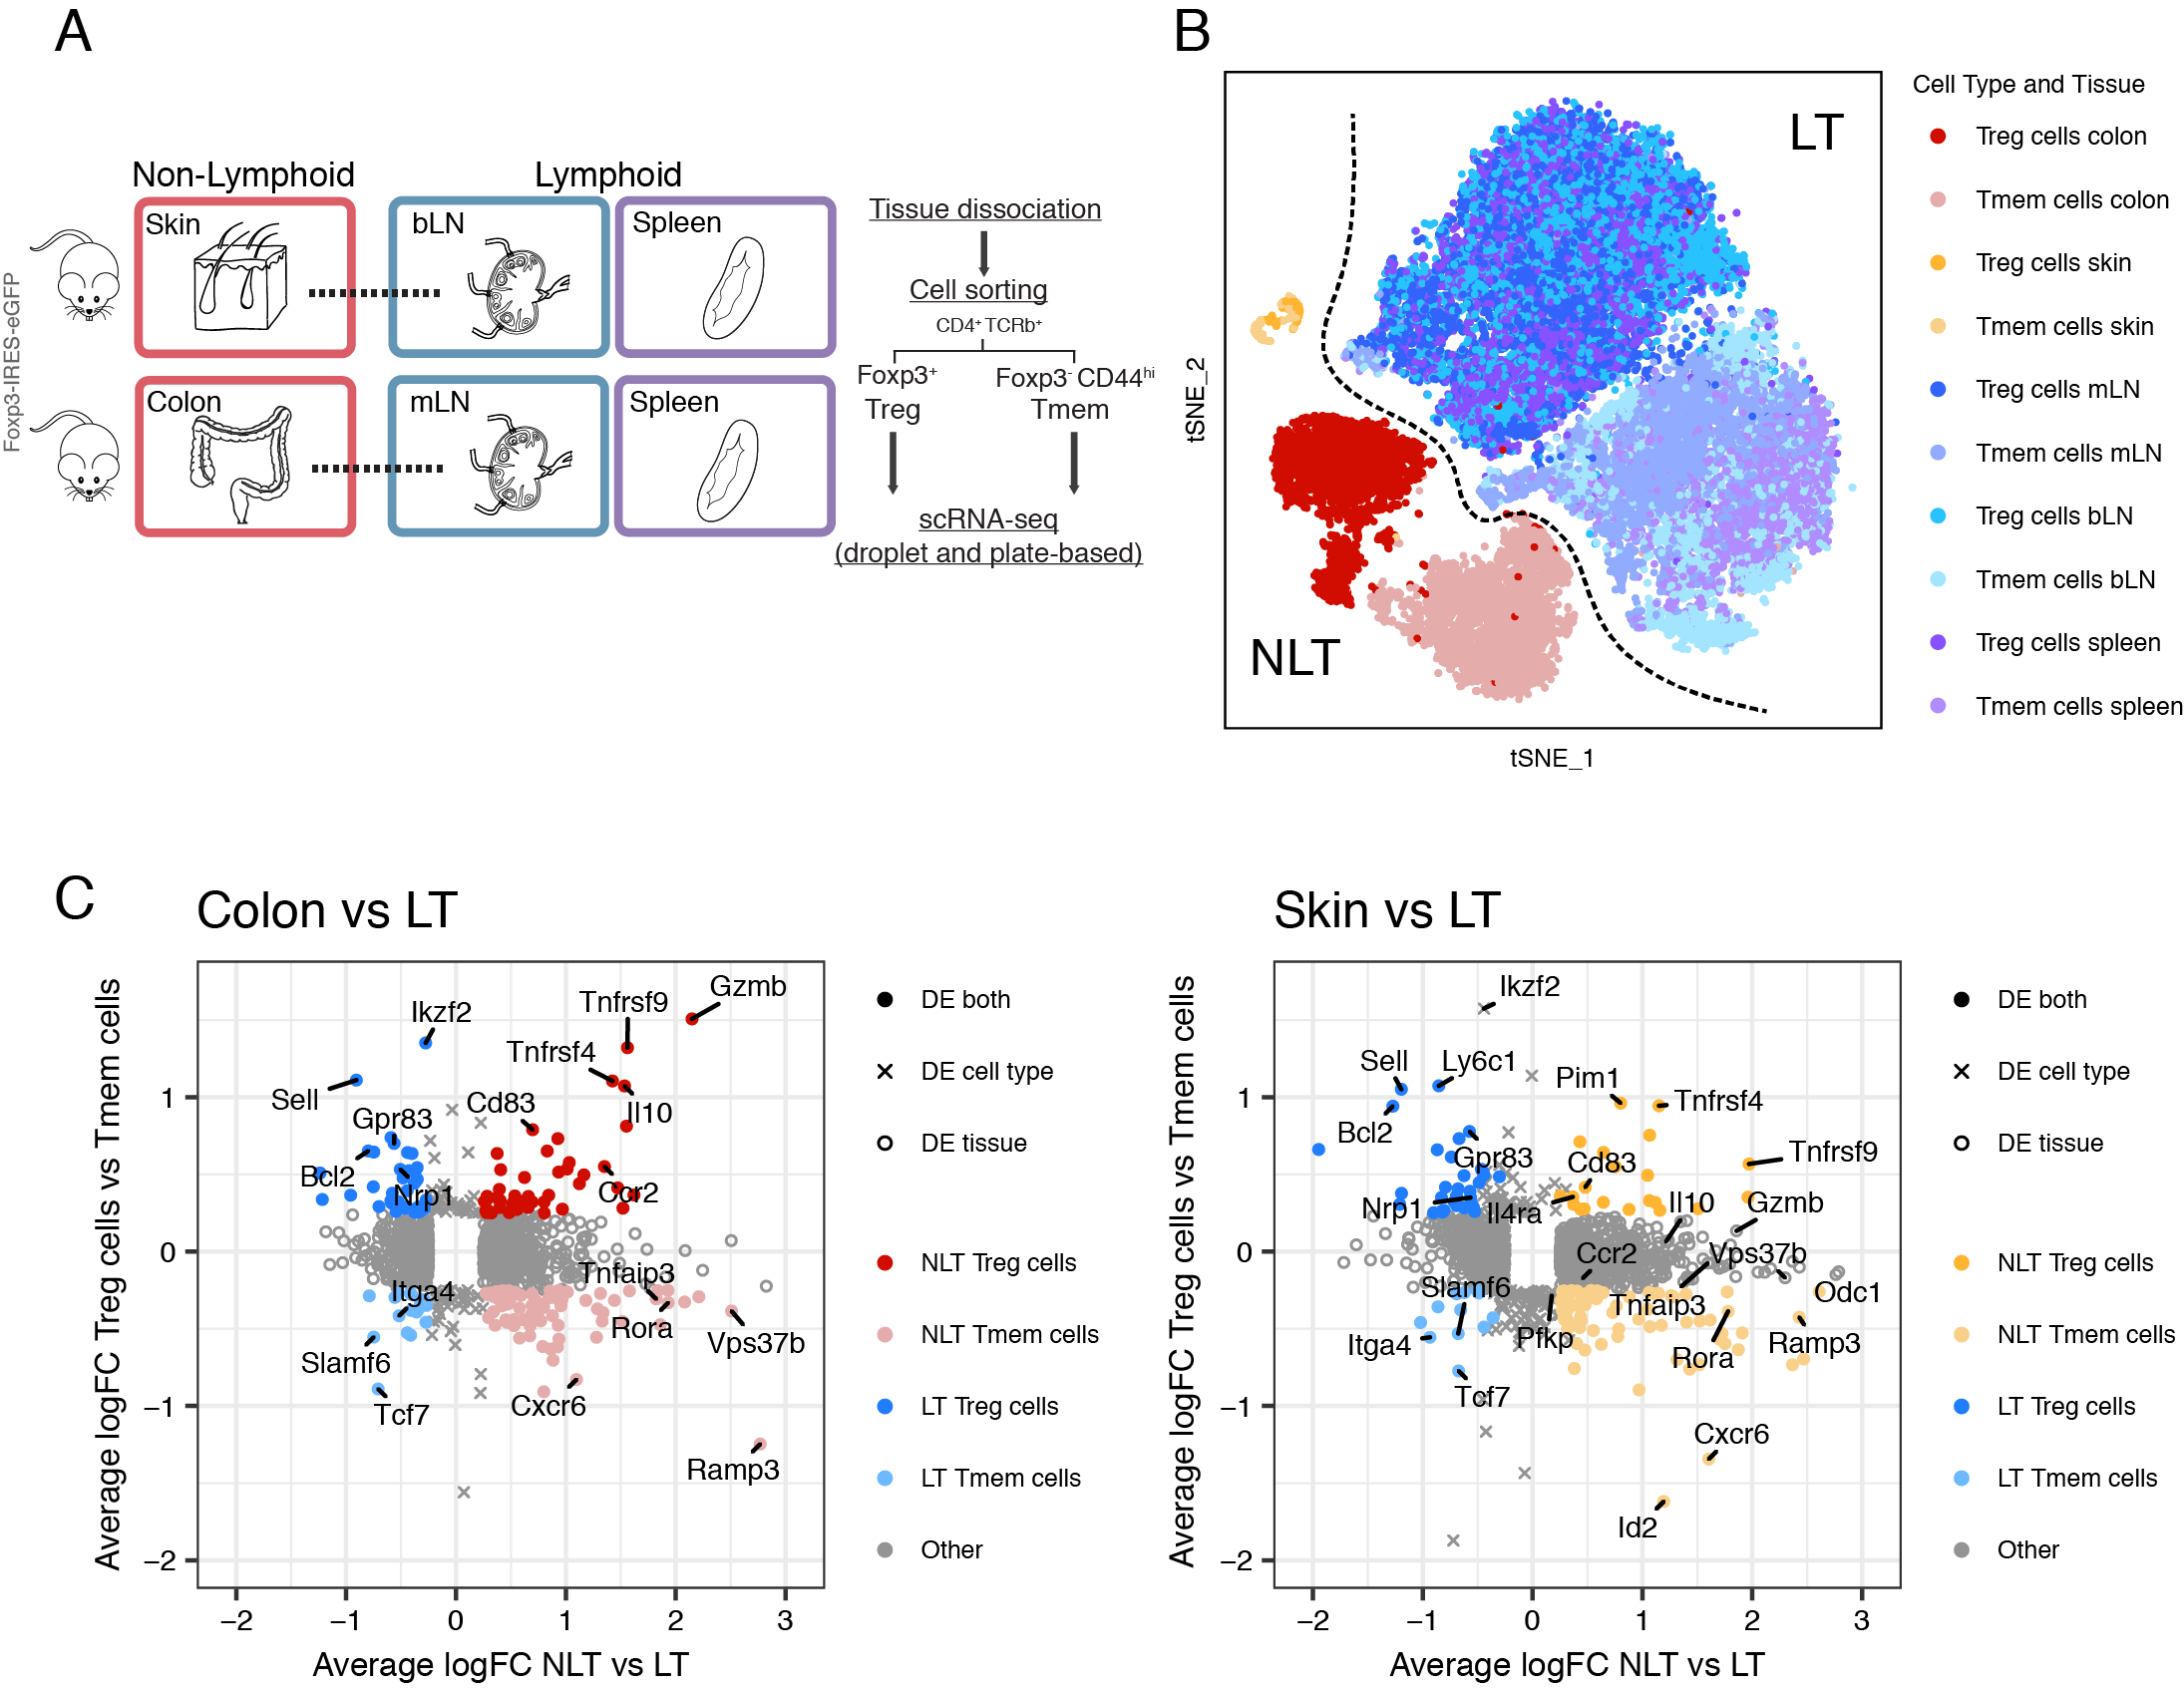
\includegraphics[width=1.0\textwidth]{Chapter2/chap2_fig1.png} % change word in curlies to change figure
\caption[chap2fig1]{(A) Experimental design for scRNA-seq data collection. (B) t-SNE representing all Treg and Tmem cells that passed quality control. (C) Genes defining the identity of Treg and Tmem cells in lymphoid and non-lymphoid tissues. Colon and skin were individually compared with their corresponding draining lymph node and spleen cells. See also Figure S1.}
\label{fig:chap2_fig1}
\end{figure}



\section[Results2]{Heterogeneity within LT and NLT Treg cell populations reflects distinct degrees of commitment to the peripheral phenotype}
\label{section2.3}

Treg cell phenotypical and functional heterogeneity has been extensively discussed in recent years (Josefowicz, Lu, and Rudensky 2012; D. J. Campbell and Koch 2011). Clustering our data within each tissue grouped Treg cells into distinct subpopulations (Figure 2A) with clearly defined marker genes (Figure 2B; Table S3). Across lymphoid organs, we identified central and effector Treg (cTreg and eTreg) cell subsets (Cretney et al. 2011; Vasanthakumar et al. 2015). cTreg cells express typical LT-associated markers, such as Tcf7, Bcl2, Sell, S1pr1, while eTreg cells expressed a subset of NLT-associated genes, like Tnfrsf9, Relb, Ikzf2 and Pdcd1. We also detected a subpopulation of Treg cells with high expression of Stat1 and interferon stimulated genes exclusively in the bLN. A fourth, less frequent population in lymphoid tissues (~5-10\%; Figure 2C), which we named Treg NLT-like cells, expresses eTreg cell markers as well as genes characteristic of NLT T cells, such as Itgae, Rora, Fgl2, Klrg1 (Figure 2B). We hypothesize that this population is primed to migrate and adapt to NLTs. Indeed, DE genes between NLT-like Treg cells from mLN and bLN revealed that the colon-homing molecules Ccr9 and Itga4, as well as their regulator Batf were upregulated specifically in the mLN, while Cxcr3 and Itgb1 were present in the bLN (Figure 2E). These differences were not observed between other LN subpopulations (data not shown).

To quantify the bias towards LT or NLT phenotypes, we calculated an NLT-LT marker gene signature for each cluster (Figure 2D; see Methods). Consistently across all LTs, cTreg cells exhibited a clear LT signature, while eTregs and NLT-like Tregs leaned towards an NLT profile, which was more pronounced in the latter. 

In the colon, we found three subpopulations of Treg cells that we labeled as NLT, suppressive and LT-like. Treg NLT and suppressive cells were present in equal proportions, both exhibiting NLT traits (Figure 2C,D). Treg NLT cells in colon express higher amounts of Gata3, Nrp1, Areg, Il1rl1, Ikzf2, matching the known thymic-derived GATA3+-subpopulation (Schiering et al. 2014)(Hu and Zhao 2015) while suppressive colonic Treg cells expressed more Il10, Gzmb, Lag3, Cxcr3, resembling the peripherally-derived RORγt+-subpopulation (Ohnmacht et al. 2015; Schiering et al. 2014; Sefik et al. 2015). Rorc itself, while not present as a marker, appears in a higher percentage of Treg suppressive cells (6.16\% vs 2.85\% in colonic Treg NLT cells). Technical limitations for detection of lowly expressed genes by scRNA-seq might account for the difficulty in capturing Rorc transcripts. Lastly, LT-like Treg cells differed from other colonic populations by expressing LT-associated genes including Sell, Ccr7, Tcf7, Bcl2, and lower amounts of NLT-associated genes such as Klrg1, Cd44, Icos, Rora, Tnfrsf9, Itgae (Figure 2B).
In contrast to the colon, and likely as a consequence of fewer cells captured, skin Treg cells did not show evident heterogeneity (Figure 2A). They expressed an unequivocal NLT signature (Figure 2D), but it was not clear to which colonic Treg cell populations they were most similar (Figure 2B). We addressed this by using a logistic regression model to calculate the probability of each skin Treg cell identifying as one of the colonic subpopulations (Figure 2G, see Methods). This revealed that most skin Treg cells were more similar to colonic Treg NLT than to Treg suppressive cells. Accordingly, colon Treg NLT cell marker genes Gata3, Il1rl1, Tnfrsf4, Rora were not differentially expressed between skin and colon Treg NLT cells (Figure 2H, Figure S2A). Despite their resemblance, differences in function and/or state between skin and colon Treg NLT might reside in a few genes. Among these are Dgat2, an enzyme involved in lipid synthesis in skin (Fagerberg et al. 2014), and Ikzf4, a transcription factor relevant for Treg stability (Sharma et al. 2013).

The same approach applied to Treg cells from the spleen, mLN and bLN (Figure 2G) classified most central and effector Treg cells as Treg LT-like cells. Treg NLT-like cells, on the other hand, were more similar to Treg NLT and Treg suppressive cells. Both the mLN and the bLN had a higher proportion of Treg cells assigned as suppressive than spleen, which contained the highest fraction of Treg NLT cells. We confirmed the presence and proportions of Treg cell subpopulations in the Smart-seq2 datasets by matching these cells to the subpopulations found across LTs and NLTs in the 10x dataset (Figure S2B).

Clustering of Tmem cells revealed multiple subpopulations (T helper-1 (Th1 cell), Th2 cells, Th17 cells, T follicular helper (Tfh) cells, lymphoid) (Figure S2C and D; Table S3) distributed differently across the tissues analysed (Figure S2D). Th1, Th2 and Th17 cells in lymphoid tissues exhibited a stronger NLT phenotype than Tmem lymphoid cells and Tfh cells (Figure S2E), which is likely an indication of their ability to adapt to and function in the NLTs.

In summary, scRNA-seq allowed us to dissect the heterogeneity of Treg cells from LTs and NLTs. We identified NLT- and LT-like Treg cell subpopulations that suggest progressive cross-tissue adaptation to the NLT environment. We found a close correspondence between skin and colonic Treg NLT cells, whilst revealing differences in gene expression that might explain their adaptation to the two environments.




% Uncomment this line, when you have siunitx package loaded.
The SI Units for dynamic viscosity is \si{\newton\second\per\metre\squared}.
I'm going to randomly include a picture Figure~\ref{fig:minion}.


If you have trouble viewing this document contact Krishna at: \href{mailto:kks32@cam.ac.uk}{kks32@cam.ac.uk} or raise an issue at \url{https://github.com/kks32/phd-thesis-template/}





\section*{Enumeration}
Lorem ipsum dolor sit amet, consectetur adipiscing elit. Sed vitae laoreet lectus. Donec lacus quam, malesuada ut erat vel, consectetur eleifend tellus. Aliquam non feugiat lacus. Interdum et malesuada fames ac ante ipsum primis in faucibus. Quisque a dolor sit amet dui malesuada malesuada id ac metus. Phasellus posuere egestas mauris, sed porta arcu vulputate ut. Donec arcu erat, ultrices et nisl ut, ultricies facilisis urna. Quisque iaculis, lorem non maximus pretium, dui eros auctor quam, sed sodales libero felis vel orci. Aliquam neque nunc, elementum id accumsan eu, varius eu enim. Aliquam blandit ante et ligula tempor pharetra. Donec molestie porttitor commodo. Integer rutrum turpis ac erat tristique cursus. Sed venenatis urna vel tempus venenatis. Nam eu rhoncus eros, et condimentum elit. Quisque risus turpis, aliquam eget euismod id, gravida in odio. Nunc elementum nibh risus, ut faucibus mauris molestie eu.
 Vivamus quis nunc nec nisl vulputate fringilla. Duis tempus libero ac justo laoreet tincidunt. Fusce sagittis gravida magna, pharetra venenatis mauris semper at. Nullam eleifend felis a elementum sagittis. In vel turpis eu metus euismod tempus eget sit amet tortor. Donec eu rhoncus libero, quis iaculis lectus. Aliquam erat volutpat. Proin id ullamcorper tortor. Fusce vestibulum a enim non volutpat. Nam ut interdum nulla. Proin lacinia felis malesuada arcu aliquet fringilla. Aliquam condimentum, tellus eget maximus porttitor, quam sem luctus massa, eu fermentum arcu diam ac massa. Praesent ut quam id leo molestie rhoncus. Praesent nec odio eget turpis bibendum eleifend non sit amet mi. Curabitur placerat finibus velit, eu ultricies risus imperdiet ut. Suspendisse lorem orci, luctus porta eros a, commodo maximus nisi.

Nunc et dolor diam. Phasellus eu justo vitae diam vehicula tristique. Vestibulum vulputate cursus turpis nec commodo. Etiam elementum sit amet erat et pellentesque. In eu augue sed tortor mollis tincidunt. Mauris eros dui, sagittis vestibulum vestibulum vitae, molestie a velit. Donec non felis ut velit aliquam convallis sit amet sit amet velit. Aliquam vulputate, elit in lacinia lacinia, odio lacus consectetur quam, sit amet facilisis mi justo id magna. Curabitur aliquet pulvinar eros. Cras metus enim, tristique ut magna a, interdum egestas nibh. Aenean lorem odio, varius a sollicitudin non, cursus a odio. Vestibulum ante ipsum primis in faucibus orci luctus et ultrices posuere cubilia Curae; 
\begin{enumerate}
\item The first topic is dull
\item The second topic is duller
\begin{enumerate}
\item The first subtopic is silly
\item The second subtopic is stupid
\end{enumerate}
\item The third topic is the dullest
\end{enumerate}
Morbi bibendum est aliquam, hendrerit dolor ac, pretium sem. Nunc molestie, dui in euismod finibus, nunc enim viverra enim, eu mattis mi metus id libero. Cras sed accumsan justo, ut volutpat ipsum. Nam faucibus auctor molestie. Morbi sit amet eros a justo pretium aliquet. Maecenas tempor risus sit amet tincidunt tincidunt. Curabitur dapibus gravida gravida. Vivamus porta ullamcorper nisi eu molestie. Ut pretium nisl eu facilisis tempor. Nulla rutrum tincidunt justo, id placerat lacus laoreet et. Sed cursus lobortis vehicula. Donec sed tortor et est cursus pellentesque sit amet sed velit. Proin efficitur posuere felis, porta auctor nunc. Etiam non porta risus. Pellentesque lacinia eros at ante iaculis, sed aliquet ipsum volutpat. Suspendisse potenti.

Ut ultrices lectus sed sagittis varius. Nulla facilisi. Nullam tortor sem, placerat nec condimentum eu, tristique eget ex. Nullam pretium tellus ut nibh accumsan elementum. Aliquam posuere gravida tellus, id imperdiet nulla rutrum imperdiet. Nulla pretium ullamcorper quam, non iaculis orci consectetur eget. Curabitur non laoreet nisl. Maecenas lacinia, lorem vel tincidunt cursus, odio lorem aliquet est, gravida auctor arcu urna id enim. Morbi accumsan bibendum ipsum, ut maximus dui placerat vitae. Nullam pretium ac tortor nec venenatis. Nunc non aliquet neque. 

\section*{Itemize}
\begin{itemize}
\item The first topic is dull
\item The second topic is duller
\begin{itemize}
\item The first subtopic is silly
\item The second subtopic is stupid
\end{itemize}
\item The third topic is the dullest
\end{itemize}

\section*{Description}
\begin{description}
\item[The first topic] is dull
\item[The second topic] is duller
\begin{description}
\item[The first subtopic] is silly
\item[The second subtopic] is stupid
\end{description}
\item[The third topic] is the dullest
\end{description}


\clearpage

\tochide\section{Hidden section}
\textbf{Lorem ipsum dolor sit amet}, \textit{consectetur adipiscing elit}. In magna nisi, aliquam id blandit id, congue ac est. Fusce porta consequat leo. Proin feugiat at felis vel consectetur. Ut tempus ipsum sit amet congue posuere. Nulla varius rutrum quam. Donec sed purus luctus, faucibus velit id, ultrices sapien. Cras diam purus, tincidunt eget tristique ut, egestas quis nulla. Curabitur vel iaculis lectus. Nunc nulla urna, ultrices et eleifend in, accumsan ut erat. In ut ante leo. Aenean a lacinia nisl, sit amet ullamcorper dolor. Maecenas blandit, tortor ut scelerisque congue, velit diam volutpat metus, sed vestibulum eros justo ut nulla. Etiam nec ipsum non enim luctus porta in in massa. Cras arcu urna, malesuada ut tellus ut, pellentesque mollis risus.Morbi vel tortor imperdiet arcu auctor mattis sit amet eu nisi. Nulla gravida urna vel nisl egestas varius. Aliquam posuere ante quis malesuada dignissim. Mauris ultrices tristique eros, a dignissim nisl iaculis nec. Praesent dapibus tincidunt mauris nec tempor. Curabitur et consequat nisi. Quisque viverra egestas risus, ut sodales enim blandit at. Mauris quis odio nulla. Cras euismod turpis magna, in facilisis diam congue non. Mauris faucibus nisl a orci dictum, et tempus mi cursus.

Etiam elementum tristique lacus, sit amet eleifend nibh eleifend sed \footnote{My footnote goes blah blah blah! \dots}. Maecenas dapibu augue ut urna malesuada, non tempor nibh mollis. Donec sed sem sollicitudin, convallis velit aliquam, tincidunt diam. In eu venenatis lorem. Aliquam non augue porttitor tellus faucibus porta et nec ante. Proin sodales, libero vitae commodo sodales, dolor nisi cursus magna, non tincidunt ipsum nibh eget purus. Nam rutrum tincidunt arcu, tincidunt vulputate mi sagittis id. Proin et nisi nec orci tincidunt auctor et porta elit. Praesent eu dolor ac magna cursus euismod. Integer non dictum nunc.


\begin{landscape}

\section*{Subplots}
I can cite Wall-E (see Fig.~\ref{fig:WallE}) and Minions in despicable me (Fig.~\ref{fig:Minnion}) or I can cite the whole figure as Fig.~\ref{fig:animations}


\begin{figure}
  \centering
  \begin{subfigure}[b]{0.3\textwidth}
    
\includegraphics[width=\textwidth]{TomandJerry}
    \caption{Tom and Jerry}
    \label{fig:TomJerry}   
  \end{subfigure}             
  \begin{subfigure}[b]{0.3\textwidth}
    
\includegraphics[width=\textwidth]{WallE}
    \caption{Wall-E}
    \label{fig:WallE}
  \end{subfigure}             
  \begin{subfigure}[b]{0.3\textwidth}
    
\includegraphics[width=\textwidth]{minion}
    \caption{Minions}
    \label{fig:Minnion}
  \end{subfigure}
  \caption{Best Animations}
  \label{fig:animations}
\end{figure}


\end{landscape}
